\documentclass[oneside]{VUMIFPSkursinis}
\usepackage{algorithmicx}
\usepackage{algorithm}
\usepackage{algpseudocode}
\usepackage{amsfonts}
\usepackage{float}
\usepackage{amsmath}
\usepackage{bm}
\usepackage{caption}
\usepackage{color}
\usepackage{float}
\usepackage{graphicx}
\usepackage{listings}
\usepackage{subfig}
\usepackage{ltablex}
\usepackage{longtable}
\usepackage{wrapfig}
\usepackage{subfig}
\usepackage{pbox}
\renewcommand{\labelenumii}{\theenumii}
\renewcommand{\theenumii}{\theenumi.\arabic{enumii}.}
\renewcommand{\labelenumiii}{\theenumiii}
\renewcommand{\theenumiii}{\theenumii\arabic{enumiii}.}
\newcolumntype{P}[1]{>{\centering\arraybackslash}p{#1}}
\usepackage[%  
    colorlinks=true,
    linkcolor=black
]{hyperref}
\university{Vilniaus universitetas}
\faculty{Matematikos ir informatikos fakultetas}
\department{Programų sistemų katedra}
\papertype{Programų sistemų inžinerija II laboratorinis darbas II}
\title{Reikalavimų apibrėžimas}
\titleineng{Requirements specification}
\status{2 kurso 3 grupės studentai}



\supervisor{Audronė Lupeikienė, M. Darbuot., Dr.}
\date{Vilnius – \the\year}

\bibliography{bibliografija}

\begin{document}
\maketitle
\tableofcontents

\section{Anotacija}
	\begin{itemize}
		\item Matas Savickis
		\item Greta Pyrantaitė
		\item Justas Tvarijonas
		\item Rytautas Kvašinskas
		\item Tomas Kiziela
	\end{itemize}

\section {Reikalavimai}

\subsubsection{Pataisyta funkcinių reikalavimų specifikacija}
\begin{enumerate}
	\item Sistema seka vartotojų laiką, praleistą trasoje, pasinaudodama sekimo prietaisu.
	\item Sistema suteikia galimybę vartotojui įsidėti pinigų į virtualią piniginę.
	\begin{enumerate}
		\item Top-up metodu.
		\item Pervedimo būdu.
	\end{enumerate}
	\item Sekimo prietaisas fiksuoja greičiausią laiką, per kurį vartotojas įveikė trasą.
	\begin{enumerate}
		\item sistema saugo greičiausią laiką, per kurį vartotojas įveikė trasą.
	\end{enumerate}
	\item Vartotojo trasų laikai rodomi internetinėje aplikacijoje.
	\item Sistema suteikia vartotojui galimybę tvarkyti savo paskyrą.
	\begin{enumerate}
		\item Prisijungti.
		\item Atsijungti.
		\item Keisti asmeninius duomenis.
		\item Keisti paskyros slaptažodį.
	\end{enumerate}
	\item Sistema internetinės aplikacijos pagalba vartotojui suteikia galimybę peržiūrėti orus.
	\begin{enumerate}
		\item Sistema turi pateikti dabartines oro sąlygas.
		\item Sistema turi pateikti ateinančių dienų orų prognozę.
		\begin{enumerate}
			\item temperaturą.
			\item drėgmę.
			\item kritulius.
			\item vėjo greitį.
		\end{enumerate}
	\end{enumerate}
	\item Internetinėje aplikacijoje vartotojas gali rašyti žinutes kitiems kurorto svečiams, administracijai ir maisto į kambarį tarnybai.
	\item Sistema vartotojui suteikia galimybę rašyti atsiliepimą apie jo viešnagę kurorte ir skirti viešą vertinimą kurortui.
	\item Internetinė aplikacija administratoriui suteikia galimybę tvarkyti duomenis.
	\begin{enumerate}
		\item Tvarkyti trasų duomenis.
		\item Tvarkyti kurorto statistinius duomenis.
		\item Tvarkyti atsiliepimus.
	\end{enumerate}
	\item Internetinė aplikacija suteikia vartotojui galimybę peržvlegti statistiką.
	\begin{enumerate}
		\item Vartotojas turi galėti peržiūrėti savo statistiką.
		\item Vartotojas turi galėti peržiūrėti kurorto statistiką, jeigu ji patvirtinta administratoriaus.
		\begin{enumerate}
			\item Administratorius turi galėti patvirtinti arba atmesti naują statistiką apie kurortą.
		\end{enumerate}
	\end{enumerate}
	\item Sistemoja per internetinę aplikaciją vartotojui suteikia galimybę peržiūrėti paslaugų kainas, tiekėjų sąrašą ir kiekvienos įrangos technines charakteristikas.
	\item Sistema administratoriui suteikia galimybę skaityti sutarčių ataskaitas.
	\item Sistema per aplikaciją vartotojui suteikia galimybę užsisakyti paslaugas.
	\begin{enumerate}
		\item Užsisakyti maisto į viešbučio kambarį.
		\item Rezervuoti slidinėjimo įrangą.
	\end{enumerate}
	\item Sistema internetinės aplikacijos pagalba leidžia vartotojui peržiūrėti visas jo pasirašytas sutartis.
	\item Vartotojas turi galimybę per internetinę aplikaciją užrezervuoti slidinėjimo trasą nurodant: trasos pavadinimą, telefono numerį, slidinėtojų skaičių ir rezervacijos laikotarpį.
	\item Vartotojas gali matyti informaciją apie slidinėjimo trasą: pavadinimą, sunkumą, rūšį, nuomos kainą, užimtumą.
	\item \textit{Sistema vartotojui suteikia galimybę peržiūrėti jo užsakytas paslaugas}
	\item \textit{Sistema administratoriui suteikia galimybę pamatyti trasas rezervavusių žmonių sąrašą}
	
	\item Sistema suteikia galimybę keisti vertinimą.
\end{enumerate}

\subsubsection{Pataisyta nefunkcinių reikalavimų specifikacija}
\begin{enumerate}

	
	\item Sistema neleidžia vertinti kurorto kelis kartus tam pačiam asmeniui dažniau, nei kartą per 2 mėnesius.

	\item Atsiskaitinėjant vartotojas gali identifikuotis piršto antspaudu.
	\item Sistema leidžia vartotojui už paslaugas atsiskaityti e-bankininkyste.
	\item Slidinėjimo trasų įrangos bei kambarių pavadinimams maksimaliai skiriama 64 simboliai
	\item Slidinėjimo trasos ilgis vaiduojamas vieno skaičiaus po kablelio tikslumu
	\begin{enumerate}
		\item Ilgio matavimo vienetas - kilometras
	\end{enumerate}
	\item Slidinėjimo trasos statumas vaizduojamas vieno skaičio po kablelio tikslumu
	\begin{enumerate}
		\item Statumo matavimo vienetas - procentai
	\end{enumerate}
	\item Slidinėjimo trasų, įrangos bei apgyvendinimo įstaigos laisvų vietų skaičius rodomas vienetų tikslumu.
	\item Slidinėjimo trasų, įrangos bei apgyvendinimo įstaigos kainos pateikiamos centų po kablelio tikslumu (10,11eu)
	\item Data turi būti vaizduojama formatu YYYY-MM-DD
	\begin{enumerate}
		\item YYYY - metai
		\item MM - mėnuo
		\item DD - diena
	\end{enumerate}
	\item Laikas turi būti vaizduojamas formatu hh:mm 24 valandų formatu (21:47)
	\begin{enumerate}
		\item hh - valandos 24 valandų formatu
		\item mm - minutės
	\end{enumerate}
	\item Vartotojo vardui, pavardei, elektroniniam paštui, slaptažodžiui registracijos formoje maksimaliai skiriama 64 simboliai. Taip pat registracijos formoje vartotojams reikia įvesti slaptažodį, kuriam maksimaliai skiriama 512 simboliai.
	\item Vartotojo raktas sugeneruojamas pagal GUID
	\item Vartotojo elektroniniam paštui prisijungiant skiriama 64 simboliai o slaptažodžiui 512
	\item Vartotojo slaptažodis negali būti trumpesnis negu 10 simbolių
	\item Vardui, pavardei ir elektroniniam paštui rezervacijos formoje skiriama 64 simboliai
	\item Telefono numeriui rezervacijos formoje skiriama 15 simbolių
	\item Svečių skaičiui rezervacijos formoje maksimaliai skiriama 3 skaičiai
	\item Orų temperatūra rodoma vienetų tikslumu. Matavimo vienetas - celsijus
	\item Rezervacijos/užsakymo/sutarties numeris pateikiamas vienetų tikslumu
	\item Įrangos dydžiai - europietiški. Vaizduojama vienetų tikslumu
	\item Keičiant naršyklės dydį, tinklapio vaizdas pritaikomas automatiškai(Responsive design).
	\item Sistema turi veikti 95proc laiko per dieną. Tai yra leidžiama neveikti 1 valandą 10 min.	
	\item Registruojant naują vartotoją sistema turi patikrinti, ar teisingai įvesti jo duomenys.
	\item Prisijungiant vartotojui sistema turi patikrinti, ar įvesti duomenys teisingi.
	\item Vartotojui rezervuojant paslaugas sistema turi patikrinti, ar duomenys įvesti korektiškai
	\item Vartotojui rezervuojant paslaugas sistema rezervacijai turi priskirti unikalų numerį.
	\item Modifikuojama tinklapio atsarginė kopija po kiekvieno informacijos atnaujinimo apie slidinėjimo kurortą, orų prognozes, slidinėjimo trasas, įrangą, apgyvendinimo įstaigą, jų užimtumą bei po kiekvienos esybės registracijos ir įvestos informacijos pakeitimo.
	\item Bandant pildyti laukus ne pagal pateiktus reikalavimus, užklausa negali būti įvykdyta.
	\item Sistemoje turi būti įdiegtos apsaugos priemonės nuo duomenų sugadinimo, praradimo, klaidingų duomenų įvedimo į duomenų bazėje.
	\item Po kiekvienos sėkmingos operacijos pakeitimai turi būti išsaugoti duomenų bazėje.
	\item Nepavykus prisijungti arba negavus duomenų iš duomenų bazės, sistema turi informuoti vartotoją, parodydamas klaidos pranešimą
	\item Didžiausia leistina tinklalapio apkrova yra 10000 vartotojų vienu metu
	\item Tinklalapio didžiausias leistinas reakcijos laikas, neįvertinant interneto greičio, turi būti ne didesnis kaip 2 sekundės.
	\item Užklausos vykdymo laikas turi būti ne didesnis nei 3 sekundės
	\item Konkrečios slidinėjimo trasos, įrangos, kambario, jų užimtumo paieškai duomenų bazėje turi būti sugaišta ne ilgiau nei 3 sekundės
	\item Tinklapis pasiekiamas prisijungiant iš bet kurio IP adreso
	\item Pradinėje sistemoje turi būti administratoriaus prisijungimo duomenys
	\item Pasirinkimų lentelė turi turėti bent 5 pradines užpildytas eilutes su informacija apie slidinėjimo trasas, įrangą, kambarius. Šią informaciją įveda įgaliotas įmonės administratorius interfeisu.
	\item Sistemos turi funkcionuoti lietuvių ir anglų kalbomis
	\item Įmonės darbuotojai turi būti apmokomi naudotis sistema
	\item Tinkalpyje negali būti klaidinančios informacijos
	\item Pakeitimai turi būti įvykdyti ne vėliau nei per 7 darbo dienas po sėkmingo testavimo.
	\item Visi vartotojo atliekami veiksmai turi būti saugomi laikinoje duomenų bazėje, kad atradus klaidą tinklalapyje būtų galima testavimo metu atkurti konkrečia klaidą
	\item Pastebėtos ar esybės praneštos klaidos turi būti ištaisytos kaip galima greičiau.
	\item Į vartotojo atsiųstus laiškus su pastebėjimai ir skundais reikia atsakyti automatine žinute.
	\item Sistema atnaujinti reikia tuo metu, kai yra mažiausias vartotojų srautas
	\item Internetinė aplikacija turi veikti bet kuriame įrenginyje, kuris turi naršyklę, palaikančią HTML5 standartą.
	\item Vartotojui prisijungiant prie sistemos vykdoma jo indentifikacija.
	\item Duomenų bazėje saugomas slaptažodžių maišos kodas, sumaišytas SHA512 algoritmu.
	\item Visi duomenys apie sistemą saugomi duomenų bazėje, o prie jos prieigą turi tik įgalioti asmenys.
	\item Atsarginė duomenų bazės kopija turi būti daroma reguliariai kas 7 darbo dienas.
	\item Jeigu esybė neaktyvi ilgiau nei 15 minučių, vartotojas automatiškai atjungiamas.
	\item Kuriant sistemą projekto komandai draudžiama naudotis nelegalia programine įranga
	\item Duomenų perdavimas ir saugojimas neturi pažeisti LR asmens duomenų teisinės apsaugos įstatymo.
	\item Esybių asmeniniai duomenys turi būti įslaptinti t.y. tinklapyje negali būti saugomi nekoduoti duomenys

\end{enumerate}


\pagebreak

\subsection{Pataisytas dalykinės srities diagrama}
\begin{figure}[h]
    \centering
    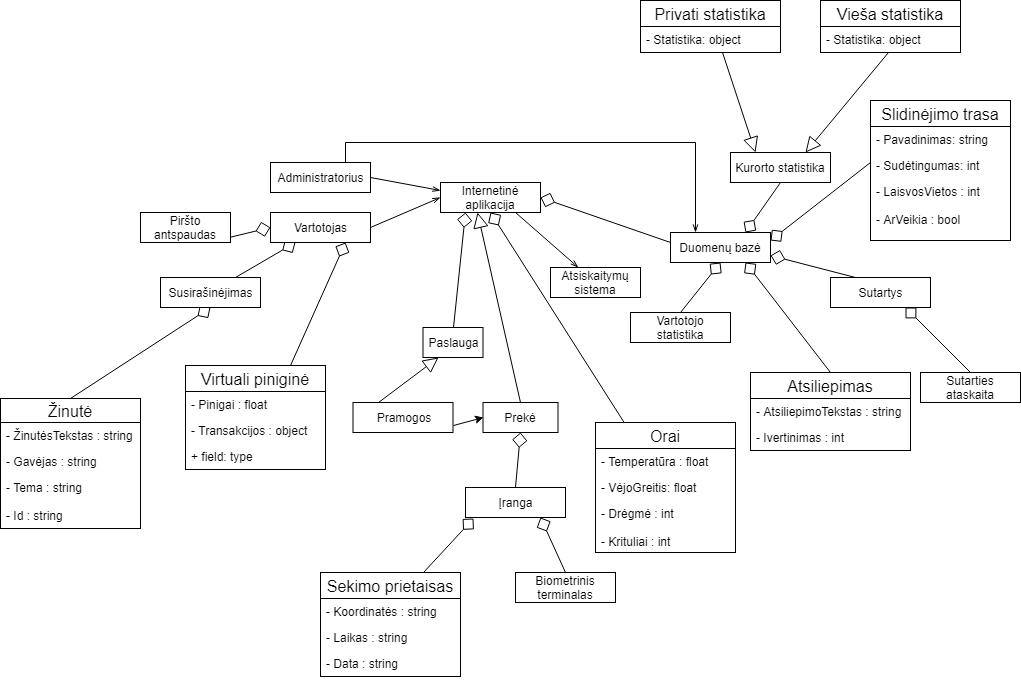
\includegraphics[width=0.80\textwidth]{DomainModelFixed.png}
    \caption{Pataisyta dalykines srities diagrama}
    \label{fig:Pataisyta dalykinės srities diagrama}
\end{figure}
\subsection{Use case peržiūra}

\section{Dalykinė sritis}
\subsection{Dalykinės srities žodynas}

\begin{enumerate}
	\item Internetinė aplikacija - Mūsų kuriama android programėlė
	\item Administratorius - Sistemą prižiūrintis žmogus
	\item Vartotojas - Slidinėjimo kurorto klientas, naudojantis programėlę
	\item Susirašinėjimas - Dviejų vartotojų žinučių grandinė
	\item Žinutė - Simbolių rinkinys, kurį vienas vartotojas siunčia kitam
	\item Virtuali piniginė - Piniginė, kurioje esančiais pinigais galima atsiskaityti už pramogas
	\item Kaina - Pinigų suma už prekę ar paslaugą
	\item Sekimo prietaisas - Įrenginys, siunčiantis savo poziciją sistemai
	\item Biometrinis terminalas - Įrenginys, kuris skenuoja piršto antspaudą
	\item Tiekėjai - Žmonės, kurie tiekia įrangą
	\item Orai - Informacija apie orų prognozę
	\item Atsiskaitymų sistema - Sistema, kuri apdoroja bankinius pinigų pervedimus
	\item Duomenų bazė - Organizuota duomenų struktūra
	\item Vartotojo statistika - Duomenys, renkami apie vartotoją
	\item Atsiliepimas - Simbolių rinkinys, parašytas vartotojo apie aplikaciją
	\item Sutartys - Rašytinis susitarimas tarp vartotojo ir slidinėjimo kurorto
	\item Slidinėjimo trasos - Informacija apie slidinėjimo trasas
	\item Kurorto statistika - Duomenys renkami apie kurortą
\end{enumerate}
\pagebreak

\subsection{dalykinies srities modelio diagrama}
\begin{figure}[h]
    \centering
    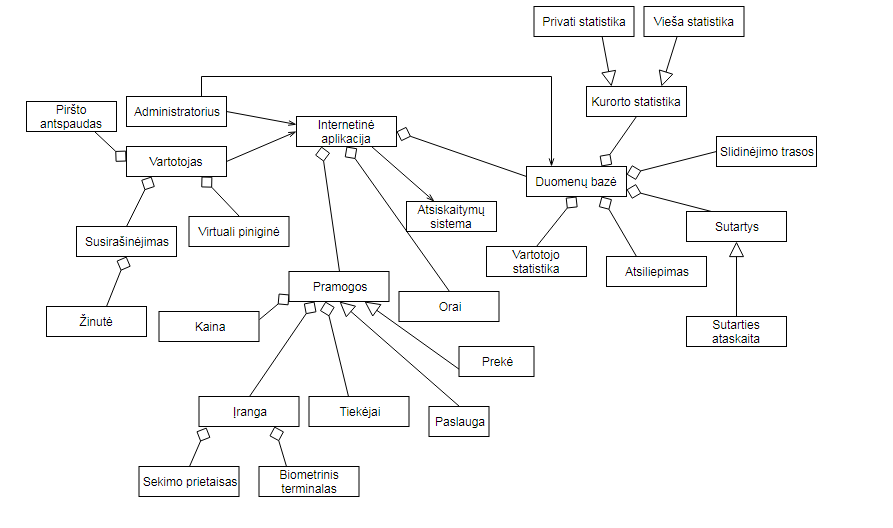
\includegraphics[width=1\textwidth]{DomainModel.png}
    \caption{Domain model diagrama}
    \label{fig:DomainModel}
\end{figure}
\pagebreak

\subsection{Reikalavimų/esybių atsekamumo matrica}	
\begin{figure}[h]
    \centering
    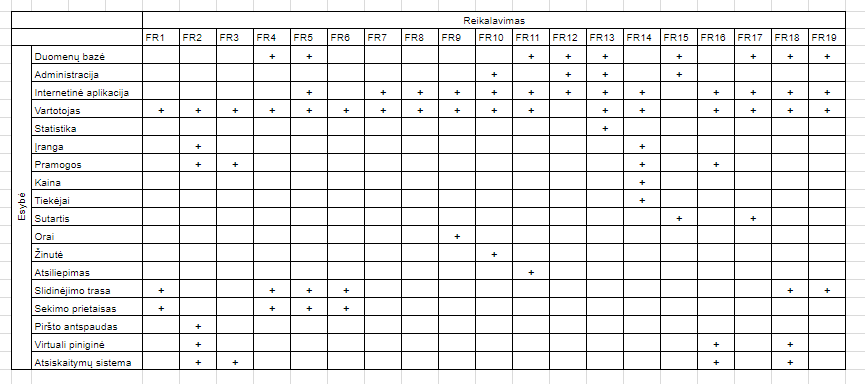
\includegraphics[width=1\textwidth]{Reikalavimai_Esybes.png}
    \caption{Reikalavimų/Esybių atsekamumo matrica}
    \label{fig:r/e_matrica}
\end{figure}
\section{Užduotys}
\Large{Use case diagramos}
\begin{figure}[h]
    \centering
    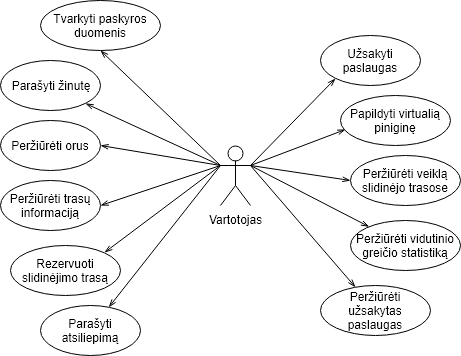
\includegraphics[width=0.75\textwidth]{useCaseVartotojas.png}
    \caption{Vartotojo užduočių diagrama}
    \label{fig:VartotojoUseCasel}
\end{figure}
\vskip 1cm
\begin{figure}[h]
    \centering
    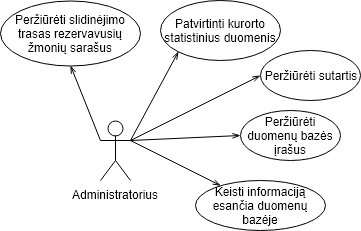
\includegraphics[width=0.65\textwidth]{useCaseAdministratorius.png}
    \caption{Administratoriaus užduočių diagrama}
    \label{fig:AdministratoriausUseCase}
\end{figure}

\begin{figure}[h]
    \centering
    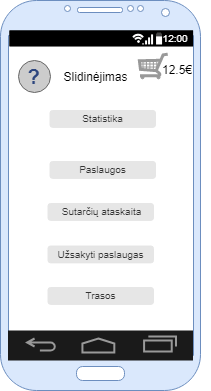
\includegraphics[width=0.30\textwidth]{mainmenu.png}
    \caption{Pagrindinio meniu langas}
    \label{fig:mainmenu}
\end{figure}

\subsection{Vartotojas įsideda pinigų į virtualią piniginę}
Trigeris: Vartotojas aplikacijoje paspaudžia ant pinigų likučio ir atsidariusiame lange paspaudžia "Papildyti piniginę". \\ \\ 
Aktoriai: Vartotojas, administratorius. \\ \\
Pagrindinis scenarijus: Vartotojui pasirinkus "Papildyti sąskaitą" atsidaro langas "Mokėjimo pasirinkimas", kuriame vartotojas gali pasirinkti, kokiu būdu nori papildyti sąskaitą, bei norimą sumą(min 3€). Mokant top-up apmokėjimo būdu vartotojas nukreipiamas į šios paslaugos teikėjo puslapį, o pasirinkus pervedimą vartotojui tame pačiame lange parodoma mokėjimo informacija, naudojantis šiuo būdu pervesti pinigai virtualioje piniginėje atsiranda administratoriui patvirtinus banko pavedimą. Viską atlikęs vartotojas gali pasinaudoti lango apačioje esančiu mygtuku "Grįžti" ir patekti atgal į pagrindinį meniu. \\ \\
Alternatyvūs scenarijai: \\ \\ 
1. Vartotojas atlieka visus nurodytus žingsnius, papildymą atlikdamas bankinio pervedimo būdu, tačiau po 3 darbo dienų jo virtuali piniginė dar nepasipildė, tuo atveju   vartotojas spaudžia klaustuką aplikacijos pagrindiniame lange, jį paspaudus atsidaro langas "Pagalba", kuriame jis nusiunčia atitinkamą pranešimą, prisegdamas pavedimo išrašo kopiją, jam kuo skubiau atrašo administratorius. \\ \\
2. Vartotojas atlieka visus nurodytus žingsnius, papildymą atlikdamas top-up būdu, tačiau mokėjimo metu dingsta prieiga prie interneto, tuo atveju tas papildymo procesas atšaukiamas ir vartotojui kitą kartą prisijungus tenka visą procesą pradėti nuo pradžių. \\ \\
\begin{figure}[h]
    \centering
    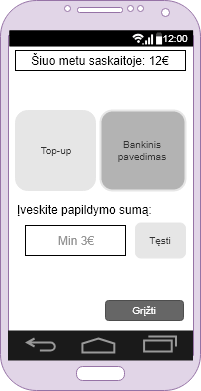
\includegraphics[width=0.20\textwidth]{Mokejimo_Pasirinkimas.png}
    \caption{Mokėjimo pasirinkimo langas}
    \label{fig:apmokejimas}
\end{figure}
\subsection{Vartotojas peržiūri savo mėnesio veiklą slidinėjimo trasose}
Trigeris: Vartotojas aplikacijoje paspaudžia mygtuką "Statistika", atsidaro langas "Vartotojo statistika", jame vartotojas pasirenka mygtuką "Mano trasų istorija" \\ \\
Aktoriai: Vartotojas \\ \\
Pagrindinis scenarijus: Vartotojas paspaudžia mygtuką "Mano trasų istorija", atsidaro langas "Vartotojo istorija", šiame lange vartotojui tinklelio pavidalu(po du eskizus horizontaliai) pavaizduotos trasos(su pavadinimais), kuriose vartotojas lankėsi per paskutinias 30 dienų, jam paspaudus ant norimos trasos iššoka pop-up langas, kuriame išrašyta vartotojo vidutinis greitis, greičiausias laikas, bei visas praleistas laikas toje trasoje. Susipažinęs su informacija vartotojas spaudžia mygtuką "Gerai", taip pašalindamas pop-up langą ir sugrįždamas į  langą "Vartotojo istorija", kurio apačioje yra mygtukas, suteikiantis galimybę grįžti į pagrindinį meniu. \\ \\
Alternatyvūs scenarijai: \\ \\
1. Vartotojas paspaudžia mygtuką "Mano trasų istorija", tačiau per pastarąjį mėnesį jis nebuvo jokioje trasoje, sistema jam parodo atitinkamą pranešimą ir nukreipia atgal į pagrindinį aplikacijos langą. \\
2. Vartotojas paspaudžia mygtuką "Mano trasų istorija", tačiau tuo metu neturi prisijungimo prie interneto, tuo atveju išvedamas pranešimas, kad norint pamatyti šią informaciją reikalingas interneto ryšys. Vartotojas nukreipiamas į pagrindinį meniu. \\
\subsection{Vartotojas peržiūri vidutinį greitį pasirinktoje trasoje}
Trigeris: Vartotojas aplikacijoje paspaudžia mygtuką "Statiska", atsidaro langas "Vartotojo statistika", jame vartotojas pasirenka "Vidutinis greitis" mygtuką. \\ \\
Aktoriai: Vartotojas. \\ \\ 
Pagrindinis scenarijus: Vartotojui pasirinkus mygtuką "Vidutinis greitis" atsidaro langas "Vidutiniai greičiai", kuriame vartotojas įveda norimos trasos pavadinimą(įvedus 3 pirmas raides sistema pasiūlo galimai tinkamus variantus), bei laikotarpį, kurio vidutinį greitį nori peržiūrėti, bei spaudžia mygtuką "Peržiūrėti". Vartotojui parodoma lentelė, kurioje surašyti kitų vartotojų vid. laikai toje trasoje, bei paryškintai rodomas vartotojo vidutinis laikas, bei šalia šios lentelės parodomas paprastas pasirinktos trasos eskizas. Lango apačioje, dešiniajame kampe vartotojas gali paspausti mygtuką "Grįžti", norėdamas patekti atgal į pagrindinį meniu. \\ \\
Alternatyvūs scenarijai: \\ \\
1. Vartotojas veda trasos pavadinimą, tačiau tokia trasa kurorte neegzistuoja, tuo atvėju vartotojui pranešame, kad tokios trasos rasti nepavyko, bei pasiūloma pasitikslinti trasos pavadinimą, bei bandyti dar kartą. \\ \\
2. Vartotojas suveda trasos pavadinimą, bei norimą laikotarpį, tačiau patikrinus aptinkama, kad šiuo laikotarpiu vartotojas joje nebuvo. Tuo atveju jam parodomas atitinkamas pranešimas ir į ekraną išvedama lentelė, kurioje yra surašyti kitų vartotojų vidutiniai laikai. Vartotojas gali grįžti į pagrindinį meniu paspaudęs mygtuką "Grįžti", esantį lango apačioje, dešinėje pusėje. \\ \\
\begin{figure}[h]
\centering
\parbox{5cm}{
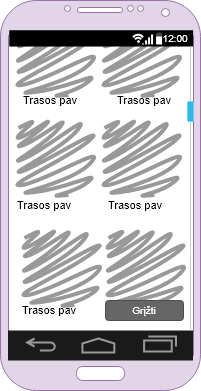
\includegraphics[width=4cm]{ManoTrasuIstorija.png}
\caption{Vartotojo trasų istorija}
\label{fig:2figsA}}
\qquad
\begin{minipage}{5cm}
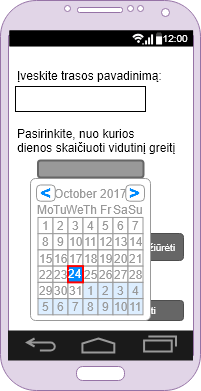
\includegraphics[width=4cm]{VidutiniaiGreičiai.png}
\caption{Vidutiniai greičiai}
\label{fig:2figsB}
\end{minipage}
\end{figure}


\subsection{Paslaugų peržiūra}
	Trigeris: Vartotojas aplikacijoje paspaudžia mygtuką "Paslaugos" ir jam atidaromas langas "Paslaugų peržiūra" \\
	Pagrindis scenarijus: Vartotojas internetinėje aplikacijoje pasirenka peržiūrėti paslaugas. Sistema vartotoją nukelią į kitą aplikacijos langą "Paslaugų peržiūra", kuriame vartotojui suteikiamas pasirinkimas peržiūrėti paslaugas arba kurorte naudojamą techniką. Tiek paslaugos, tiek technika pateikiama sąrašu, prie kiekvieno sąrašo elemento yra paveiksliukas, atitinkantis konkrečią paslaugą, ir paslaugos ar įrangos pavadinimas. Vartotojas gali paspausti ant kiekvieno sąrašo elemento, norėdamas sužinoti detalesnę informaciją \\ \\
Alternatyvūs scenarijai:\\ \\
1. Sistema negali pateikti paslaugų sąrašo. Vartotojui parodomas informacinis pranešimas, kad vyksta techniniai darbai ir pasiūloma sugrįžti vėliau. Vartotojui suteikiama galimybė grįžti į pagrindinį aplikacijos langą.\\
2. Nėra detalesnės informacijos apie paslaugą arba įrangą. Vartotojui parašoma, kad papildomos informacijos nėra ir pasiūloma susisiekti su klientų aptarnavimo skyriumi dėl detalesnės informacijos. Vartotojui parodomas aptarnavimo skyriaus elektroninis paštas ir suteikiama galimybė grįžti į pagrindinį aplikacijos langą.

\subsection{Administratorius peržiūri sutarčių ataskaitą}
	Trigeris: Administratorius aplikacijos suteiktoje darbo aplinkoje paspaudžia mygtuką "Sutarčių ataskaitos" ir jam atidaromas langas "Ataskaitos"\\
	Pagrindinis scenarijus: Administratorius darbo aplinkoje pasirenka peržiūrėti sutarčių ataskaitas. Sistema iš duombazės gauna ir atvaizduoja sutarčių sąrašą lange "Ataskaitos". Kiekvienas sarašo elementas turi pavadinimą, sutarties numerį ir pasirašymo datą. Administratoriui suteikiama galimybė paspaudus ant individualaus sąrašo elemento matyti detalią konkrečios sutarties ataskaitą. Taip pat suteikiama galimybė ieškoti sutarties pagal jos numerį bei rušiuoti sutartis pagal datą\\ \\
	Alternatyvūs scenarijai: \\ \\
1. Administratoriui pasirinkus sutarčių peržiūrą sistemai nepavyksta susisiekti su duomenų baze. Administratoriui pateikiamas klaidos kodas, serverių statusas, nurodymai, kas padėtų išspręsti problemą, ir suteikiami techninės pagalbos kontaktai. \\ 
2. Administratorius į paieškos lauką įveda sutarties numerį, tačiau tokia sutartis sistemoje neegzistuoja. Parodomas informacinis pranešimas, kad tokia sutartis neegzistuoja \\ \\

\subsection{Vartotojas užsako paslaugas}
	Trigeris: Vartotojas aplikacijoje paspaudžia mygtuką "užsakyti paslaugas", atidaromas langas "Paslaugos užsakymas"\\
	Pagrindinis scenarijus: Vartotojas internetinėje aplikacijoje paspaudžia mygtuką "Užsisakyti paslaugas". Vartotojui pateikiamas paslaugų sąrašas lange "Paslaugos užsakymas" ir kiekvienos paslaugos kaina vienam žmogui. Vartotojas turi galimybę pasirinkti paslaugą ir užsakyti ją iki 10 žmonių, ir pasirinkti paslaugos laiką. Varotojui parašius žmonių skaičių ir patvirtinus užsakymą, jis atsiranda prekių krepšelyje ir paslaugos kaina pridedama prie bendros krepšelio kainos.\\ \\
	Alternatyvūs scenarijai:  \\ \\
1. Vartotojui pasirinkus užsakyti konkrečią paslaugą ir jos laiką ši paslauga tuo laiku negalima. Vartotojui parodomas pranešimas, kad paslauga tuo metu negalima. Vartotojui pateikiamas artimiausias laisvas laikas. \\ 
2. Vartotojui pasirinkus užsakyti paslaugą sistema negali nusiųsti paslaugos užsakymo užklausos. Vartotojui parodomas informacinis pranešimas, kad vyksta techniniai darbai ir paslaugų užsakyti negalima. Vartotojui paskiūloma paslaugą užsisakyti telefonu paskambinus į kurortą, užsakymą parašyti elektroniniu paštu arba sugrįžti vėliau.\\ \\

\subsection{Vartotojas peržiūri užsakytas paslaugas}
	Trigeris: Vartotojas aplikacijoje paspaudžia mygtuką "Paslaugos", atidaromas langas "Palaugos"\\
	Pagrindinis scenarijus: Vartotojas internetinėje aplikacijoje paspaudžia mygtuką "Paslaugos". Vartotojui pateikiamas jo užsakytų paslaugų sąrašas lange "Paslaugos". Vartotojui suteikiama galimybė paspaudus ant individualaus sąrašo elemento matyti detalią paslaugos informaciją.\\ \\
	Alternatyvūs scenarijai:\\ \\
1. Vartotojui pasirinkus užsakytų paslaugų peržiūrą nerandama užsakytų paslaugų. Vartotojui parodoma nuoroda užsakyti paslaugas. Vartotojui siūloma palaukti, jei neseniai užsisakė paslaugą. Vartotojui siūloma kreiptis pagalbos, jei nuo paslaugos užsakymo jau praėjo diena laiko.\\ \\
2. Vartotojui pasirinkus užsakytų paslaugų peržiūrą sistema negali susisiekti su duomenų baze. Vartotojui parodomas pranešimas, kad vyksta techniniai darbai ir pasiūloma sugrįžti vėliau. Vartotojui pateikiama nuoroda grįžti į pagrindinį puslapį.\\ \\

\begin{figure}[h]
\centering
\parbox{5cm}{
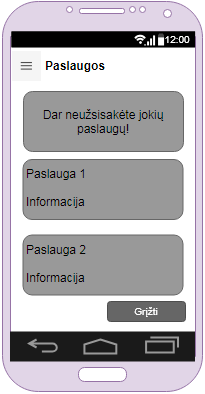
\includegraphics[width=4cm]{GUI-17-uzsakytos-paslaugos(1).png}
\caption{Vartotojas neužsisakė jokių paslaugų}
\label{fig:2figsA}}
\qquad
\begin{minipage}{5cm}
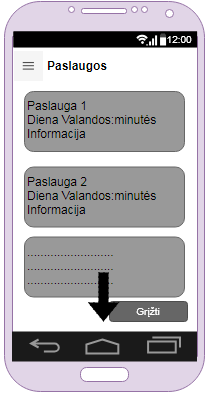
\includegraphics[width=4cm]{GUI-17-uzsakytos-paslaugos(2).png}
\caption{Paslaugos ir jų užsakymo laikas}
\label{fig:2figsB}
\end{minipage}
\begin{minipage}{5cm}
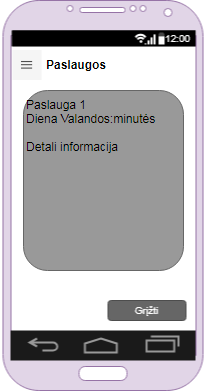
\includegraphics[width=4cm]{GUI-17-uzsakytos-paslaugos(3).png}
\caption{Detali paslaugos informacija}
\label{fig:2figsC}
\end{minipage}
\end{figure}


\subsection{Vartotojas rezervuoja trasą}
	Trigeris: Vartotojas aplikacijoje paspaudžia mygtuką ,,Trasos"\\ \\
	Aktoriai: Vartotojas\\ \\
	Pagrindinis scenarijus: Vartotojas internetinėje aplikacijoje paspaudžia mygtuką ,,Trasos". Vartotojui pateikiamas trasų sąrašas. Vartotojui suteikiama galimybė paspaudus ant individualaus sąrašo elemento matyti detalią trasos informaciją ir laisvas rezervacijai dienas bei valandas. Vartotojui pasirinkus laiką ir patvirtinus užsakymą, užsakymas pridedamas į krepšelį. Vartotojui parodomas pranešimas apie sėkmingai pridėtą užsakymą ir pasiūloma peržiūrėti prekių krepšelį.\\ \\
	Alternatyvūs scenarijai:\\ \\
1. Vartotojui besirenkant rezervacijos laiką įvyksta kitas užsakymas ir jo pasirinktas laikas tampa užimtas. Vartotojui patvirtinus užsakymą parodomas pranešimas, kad trasa tuo laiku užimta. Vartotojui pasiūloma atnaujinti langą ir pamatyti naują trasos užimtumą.\\ \\
2. Vartotojui paspaudus mygtuką ,,Trasos" trasų sąrašas yra tuščias. Vartotojui siūloma dėl trasų rezervacijos pasiteirauti telefonu ar elektroniniu paštu.\\ \\
3. Vartotojui paspaudus mygtuką ,,Trasos" sistema negali susisiekti su duomenų baze. Vartotojui parodomas pranešimas, kad vyksta techniniai darbai ir pasiūloma sugrįžti vėliau. Vartotojui pateikiama nuoroda grįžti į pagrindinį puslapį.\\ \\

\begin{figure}[h]
\centering
\parbox{5cm}{
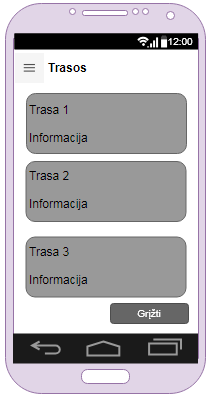
\includegraphics[width=4cm]{GUI-18-19-trasos.png}
\caption{Visos trasos}
\label{fig:2figsA}}
\qquad
\begin{minipage}{5cm}
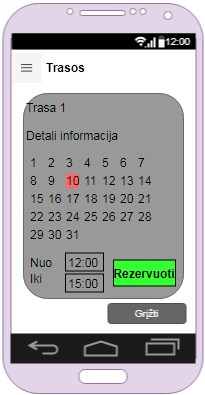
\includegraphics[width=4cm]{GUI-18-19-detali-trasos-informacija.png}
\caption{Rezervuoti trasą}
\label{fig:2figsB}
\end{minipage}
\end{figure}

\subsection{Vartotojas peržiūri informaciją apie trasą}
	Trigeris: Vartotojas aplikacijoje paspaudžia mygtuką "Trasos" ir jam atidaromas langas "Trasos"\\
	Pagrindinis scenarijus: Vartotojas internetinėje aplikacijoje paspaudžia mygtuką "Trasos". Vartotojui atidaromas langas "Trasos", kuriame pateikiamas trasų sąrašas. Vartotojui paspaudus ant individualaus sąrašo elemento parodoma detalesnė trasos informacija.\\ \\
	Alternatyvūs scenarijai:\\ \\
1. Vartotojui paspaudus ant sąrašo elemento trūksta informacijos apie trasą. Vartotojui pasiūloma pasiteirauti telefonu ar elektroniniu paštu.\\ \\
2. Vartotojui paspaudus mygtuką ,,Trasos" sistema negali susisiekti su duomenų baze. Vartotojui parodomas pranešimas, kad vyksta techniniai darbai ir pasiūloma sugrįžti vėliau. Vartotojui pateikiama nuoroda grįžti į pagrindinį puslapį.\\ \\
	
\subsection{Vartotojas peržiūri orus}
	Trigeris: Vartotojas aplikacijoje paspaudžia mygtuką "Orai", atsidaro naujas langas "Orų peržiūra" \\ \\
	Aktoriai: Vartotojas \\ \\
Pagrindinis scenarijus: Vartotojas aplikacijoje paspaudžia mygtuką "Orai". Atidaromas naujas langas "Orų peržiūra", kuriame yra du mygtukai: "Dabartiniai orai" ir "Orų prognozė".Vartotojui pasirinkus ,,Dabartinė orų prognozė" pateikiami esami orų duomenys. Pasirinkus ,,Orų prognozė" vartotojo paprašoma pasirinkt kokios dienos prognozės nori matyti. Abiejuose pasirinkimuose pateikiami šie duomenys: temperatūra, drėgmė, krituliai bei vėjo greitis. Peržiūrėjęs orus vartotojas uždaro langą, paspausdamas mygtuką "Grįžti į pagrindinį meniu". \\
	Alternatyvus scenarijus: Vartotojas paspaudžia mygtuką "Orai". Atidaromas naujas langas "Orų peržiūra", tačiau nepavyksta prisijungti prie orų API. Vartotojui parodomas pranešimas, jog nepavyko gauti orų informacijos, ir prašoma pabandyti vėliau. Vartotojas grąžinamas į pagrindinį meniu. \\ \\


\begin{figure}[h]
    \centering
    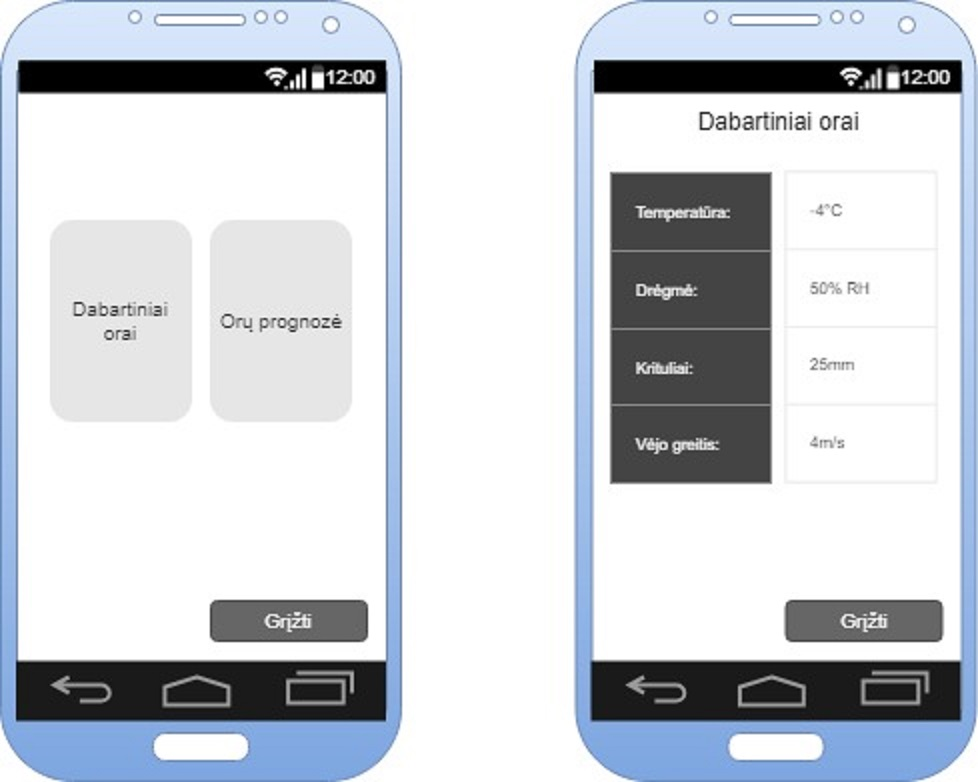
\includegraphics[width=0.80\textwidth]{GUI11.jpg}
    \caption{Orų peržiūros langas}
    \label{fig:orai}
\end{figure}


\subsection{Vartotojas rašo žinutę}
	Trigeris: Vartotojas aplikacijoje paspaudžia mygtuką "Rašyti naują žinutę", jam iššoka langas "Nauja žinutė" \\ \\
	Aktoriai: Vartotojas \\ \\
	Pagrindinis scenarijus: Vartotojas aplikacijoje paspaudžia mygtuką "Rašyti naują žinutę", jam iššoka langas "Nauja žinutė". Vartotojas pasirenka gavėją (kitas vartotojas, administratorius ar maisto į kambarį tarnyba), nurodo gavėjo vardą (jei to reikia), nurodo žinutės temą, parašo žinutę ir ją išsiunčia paspausdamas mygtuką "Siųsti žinutę". Išsiuntus žinutę vartotojui atidaromas naujas langas "Nauja žinutė", kurį jis uždaro paspausdamas mygtuką "Atgal". \\ \\
	Alternatyvus scenarijus: Vartotojas aplikacijoje paspaudžia mygtuką "Rašyti naują žinutę", jam iššoka langas "Nauja žinutė". Vartotojas pasirenka gavėją (kitas vartotojas, administratorius ar maisto į kambarį tarnyba), nurodo gavėjo vardą (jei to reikia), nurodo žinutės temą, parašo žinutę ir ją išsiunčia paspausdamas mygtuką "Siųsti žinutę", tačiau neteisingai nurodo gavėjo vardą ir žinutė neišsiunčiama. Sistema vartotojui išmeta klaidos pranešimą ir leidžia jam atlikti norimus pakeitimus. \\ \\

\subsection{Vartotojas parašo atsiliepimą}
	Trigeris: Vartotojas aplikacijoje paspaudžia mygtuką "Rašyti atsiliepimą", atsidaro naujas langas "Atsiliepimai" \\ \\
	Aktoriai: Vartotojas \\ \\
	Pagrindinis scenarijus: Vartotojas paspaudžia mygtuką "Rašyti atsiliepimą". Aplikacijoje atsidaro naujas langas "Atsiliepimai", kuriame vartotojas gali sukurti naują atsiliepimą. Vartotojas įvertina savo viešnagę 1-5 žvaigždutėm, bei atskirame laukelyje parašo savo komentarus. Baigęs rašyti savo atsiliepimą vartotojas paspaudžia mygtuką "Siųsti" ir atsiliepimas išsiunčiamas. Vartotojas paspaudžia mygtuką atgal ir grįžta į pagrindinį meniu. \\ \\
	Alternatyvus scenarijus: Vartotojas paspaudžia mygtuką "Rašyti atsiliepimą". Aplikacijoje atsidaro naujas langas "Atsiliepimai", kuriame vartotojas gali sukurti naują atsiliepimą. Vartotojas laukelyje parašo komentarus apie savo viešnagę. Baigęs rašyti savo atsiliepimą vartotojas paspaudžia mygtuką "Siųsti", tačiau vartotojas neįvertino savo viešnagės. Vartotojo paprašoma pateikti 1-5 žvaigždučių įvertinimą. Vartotojas baigęs grįžta į pagrindinį meniu paspaudęs mygtuką "Atgal". \\ \\

\begin{figure}[h]
    \centering
    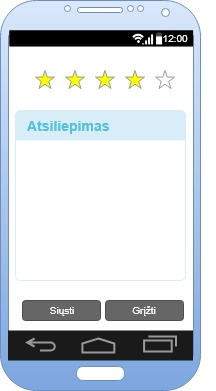
\includegraphics[width=0.30\textwidth]{GUI13.jpg}
    \caption{Atsiliepimo parašymo langas}
    \label{fig:atsiliepimas}
\end{figure}


\subsection{Administratorius peržiūri duomenų bazę}
	Trigeris: Administratorius aplikacijoje paspaudžia mygtuką "Peržiūrėti duomenų bazę", jam atidaromas duombazės peržiūros langas "Duomenų bazės peržiūra"
	Aktoriai: Administratorius
	Pagrindinis scenarijus: Administratorius paspaudžia mygtuką "Peržiūrėti duomenų bazę", jam prisijungiama prie duomanų bazės ir atidaromas duombazės peržiūros langas "Duomenų bazės peržiūra". Administratorius stebi duomenų bazėje esančių objektų būseną. Administratorius pasirenka objektą ir pakeičia jo duomenis. Padaręs pakeitimus, administratorius juo išsaugo paspaudęs mygtuką "Saugoti" ir baigęs darbą su duombaze, nuo jos atsijungia paspausdamas mygtuką "Atgal". \\ \\
	Alternatyvūs scenarijai:  \\ \\ 
1. Administratorius paspaudžia mygtuką "Peržiūrėti duomenų bazę", tačiau sistemai nepavyksta prisijungti prie duomenų bazės. Administratoriui išmetamas pranešimas, jog nepavyko prisijungti prie duomenų bazės ir paprašoma jo bandyti vėliau. Administratorius grąžinamas į pagrindinį meniu. \\
2. Administratorius paspaudžia mygtuką "Peržiūrėti duomenų bazę", jam prisijungiama prie duomanų bazės ir atidaromas duombazės peržiūros langas "Duomenų bazės peržiūra". Administratorius stebi duomenų bazėje esančių objektų būseną. Administratorius pasirenka objektą ir pakeičia jo duomenis. Padaręs pakeitimus administratorius bando atsijungti nuo duomenų bazės spausdamas mygtuką "Atgal". Sistema išmeta pranešimą, jog jo padaryti pakeitimai nėra išsaugoti ir paklausia, ar jis nori išsaugoti pakeitimus. Administratorius paspaudžia mygtuką "Taip", tada paspaudžia mygtuką "Saugoti" ir atsijungia nuo duomenų bazės paspausdamas mygtuką "Atgal", kuris grąžina jį į pagrindinį meniu. \\ \\

\subsection{Vartotojas peržiūri savo poziciją ir laiką praleistą trasoje}
	Trigeris: Vartotojas paspaudžia mygtuką ''Žemėlapis'', ir jam atidaromas langas "Žemėlapis"\\
	Pagrindinis scenarijus: Vartotojas paspaudžia mygtuką ''Žemėlapis'', atsiveria langas "Žemėlapis", kuriame yra vaizduojamos visos trasos. Raudonu tašku pažymėta vartotojo dabartinė vieta. Apačioje rodomas trasos pavadinimas, praleistas ir likęs vartotojo laikas joje. Paspaudus ant trasų pavadinimo žemėlapyje atveriamas langas su detalesne informacija apie ją.\\ \\
Alternatyvūs scenarijai:  \\ \\
1. Vartotojas paspaudžia mygtuką ''Žemėlapis'', atveriamas langas su trasų žemėlapiu, bet nerandama vartotojo dabartinė vieta. Vartotojui parodomas langas, kuriame siūloma įsijungti GPS, o alternatyviai - pagalbos telefonas.\\
2. Vartotojas paspaudžia mygtuką ''Žemėlapis'', atveriamas langas su trasų žemėlapiu. Paspaudus ant trasos pavadinimo, atveriamas naujas langas, bet trūksta informacijos jame.  Vartotojui pasiūloma pasiteirauti telefonu ar elektroniniu paštu. \\ \\ 

\subsection{Vartotojas nori pasikeisti asmeninis duomenis}
Trigeris: Vartotojas paspaudžia mygtuką ''Profilis'' ir jam atidaromas langas "Profilis" \\
	Pagrindinis scenarijus: Vartotojas paspaudžia mygtuką ''Profilis'', jam atveriamas langas "Profilis", su laukais: Vardas, Pavardė, El. paštas, Keisti slaptažodį. Galima redaguoti visus laukus. Paspaudus 'Keisti slaptažodį'' sugeneruojamas naujas raktas ir jis išsiunčiamas į jo el. paštą. Apačioje yra mygtukas ''Atsijungti''. Jį paspaudus vartotojas atjungiamas nuo sistemos ir jam atveriamas prisijungimo langas.\\
Alternatyvus scenarijus: Vartotojas paspaudžia mygtuką ''Profilis'', jam atveriamas langas su laukais: Vardas, Pavardė, El. paštas, Keisti slaptažodį.  Paspaudus ''Keisti slaptažodį'' sugeneruojamas naujas raktas ir pranešama, kad slaptažodis išsiųstas į nurodytą el. paštą. Vartotojui jo negavus, spaudžiamas mygtukas ''Siųsti iš naujo''. Išvedamas pranešimas, kad slaptažodis išsiųstas ir pasiūloma pasitikrinti  ''Spam'' folderį. \\ \\ 

\subsection{Reikalavimų - užduočių atsekamumo matrica}
\begin{figure}[h]
    \centering
    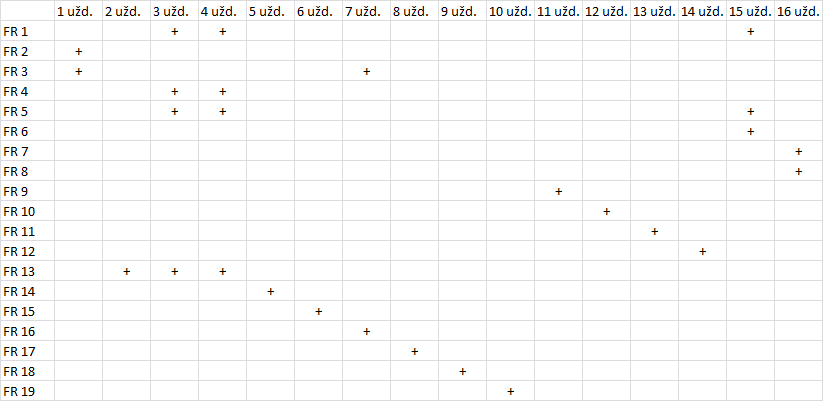
\includegraphics[width=1\textwidth]{reik_uzd_matrica_before.png}
    \caption{Reikalavimų/Užduočių atsekamumo matrica}
    \label{fig:matrica}
\end{figure}

\section{Robastiškumo analizė}

\section{Eskizinio projekto peržiūra}

\section{Techninė architektūra}


\end{document}